\documentclass[a4paper,faculty=eb,language=en,doctype=article,sftitles=false]{ugent-doc}

\usepackage[utf8]{inputenc}
\usepackage[T1]{fontenc}
\usepackage[english]{babel}
\usepackage{lmodern}
\usepackage{amsmath}
\usepackage{booktabs}
\usepackage{enumitem}
\usepackage{graphicx}
\usepackage{float}
\usepackage{xcolor}
\usepackage[hidelinks]{hyperref}
\usepackage{pgfplots}
\pgfplotsset{compat=1.18}

\setlength{\abovedisplayskip}{6pt}
\setlength{\belowdisplayskip}{6pt}
\setlength{\abovedisplayshortskip}{4pt}
\setlength{\belowdisplayshortskip}{4pt}
\setlength{\emergencystretch}{3em}
\setlength{\parindent}{0pt}

\newcommand{\assignmentsection}[1]{%
  \refstepcounter{section}%
  \section*{#1}%
  \addcontentsline{toc}{section}{#1}%
}

\newcommand{\introsection}[1]{%
  \section*{#1}%
  \addcontentsline{toc}{section}{#1}%
}

\thetitle{%
\textbf{Advanced Production Management (F000896A)}\\[0.3em]
\textbf{Project Report 2026}%
}

\infoboxa{Prof.\ Dr.\ Veronique Lim\`ere \& Hannah Verplancke}

\infoboxb{
Students:\quad Group A\\[0.5em]
\begin{tabular}{@{}lll@{}}
\hspace*{2em}JONAS PAREWYCK & \hspace*{2em}02210616 & \hspace*{2em}jonas.parewyck@ugent.be\\
\hspace*{2em}LEONARD DESMET & \hspace*{2em}02203659 & \hspace*{2em}leonard.desmet@ugent.be\\
\hspace*{2em}STEF DESENDER & \hspace*{2em}02208912 & \hspace*{2em}stef.desender@ugent.be\\
\hspace*{2em}SARE VANHOUTTE & \hspace*{2em}02211452 & \hspace*{2em}sare.vanhoutte@ugent.be\\
\hspace*{2em}MARGOT DE COCK & \hspace*{2em}02110278 & \hspace*{2em}macock.decock@ugent.be\\
\end{tabular}
}

\infoboxc{Academic year:\quad 2025--2026}

\begin{document}

\maketitle
\clearpage

\pagenumbering{gobble}
\newgeometry{left=1.5cm,right=1.5cm,top=1.8cm,bottom=1.8cm}
\tableofcontents
\clearpage

\pagenumbering{arabic}
\setcounter{page}{1}

\introsection{Introduction to the case}

This project focuses on optimizing production planning in a multi-stage manufacturing system using a Mixed Integer Programming (MIP) approach. The objective is to minimize total costs while ensuring efficient production and inventory decisions. By comparing solutions based on forecasted and realized demand, the project provides insights into the impact of uncertainty and the trade-offs between cost efficiency and service levels.

\assignmentsection{Assignment 1: Formulating an MIP model with infinite production capacity}

\subsection{Plan based on forecasted demand}

\subsubsection{Indices}

\begin{itemize}[noitemsep]
    \item $i \in parts = \{B1401, B2302, B3201, B4702, V1501, V6302, E2801\}$
    \item $t \in weeks = \{1,2,\ldots,30\}$
\end{itemize}

\subsubsection{Parameters}

The model covers $T = 30$ periods (weeks). Each part $i$ has a lead time $LT_i$ (periods between placing and receiving an order), a minimum lot size $L_i$ (minimum quantity per order) and a beginning inventory $I_{i,0}$ (initial stock at the start of the horizon). Holding costs $h_i$ apply per unit per week, while setup costs $S_i$ are incurred per order placement. Finally, $FD_{i,t}$ and $RD_{i,t}$ represent respectively the forecasted and realized demand for part $i$ in period $t$.

While the forecasted and realized demand for the end product ($E2801$) are externally driven, component demand (V1501, V6302, B1401, \ldots) is derived internally from the production schedule of their parent item. Component gross requirements are determined by the Planned Order Releases of the parent, multiplied by the Bill of Materials (BOM) factor. This demand occurs one lead time period before the parent is completed, creating a cascading effect throughout the BOM: as soon as a parent part enters production, the required components are immediately withdrawn from inventory.

\begin{table}[H]
\centering
\begin{tabular}{ll}
\toprule
\textbf{Symbol} & \textbf{Description} \\
\midrule
$T$ & forecast horizon (30 weeks) \\
$LT_i$ & lead time of part $i$ \\
$L_i$ & minimum lot size of part $i$ \\
$I_{i,0}$ & initial inventory of part $i$ \\
$h_i$ & holding cost (€ / unit / week) \\
$S_i$ & setup cost (€ / setup) \\
$FD_{i,t}$ & forecasted demand of part $i$ in period $t$ \\
$RD_{i,t}$ & realized demand of part $i$ in period $t$ \\
\bottomrule
\end{tabular}
\caption{Overview of model parameters}
\end{table}

\subsubsection{Decision variables}

Three decision variables are defined for each part $i$ and period $t$. The first, $x_{i,t}$, represents the units ordered or produced, and is continuous and non-negative. The second is $y_{i,t}$, is binary, equaling 1 when an order is initiated for part $i$ in period $t$, thereby incurring setup cost $S_i$. The third, $I_{i,t}$, is a non-negative integer representing the inventory level of part $i$ at the end of period $t$, after all receipts and withdrawals in period $t$ have been processed. A holding cost $h_i$ is charged per remaining unit in inventory at the end of each period.

\[
x_{i,t} = \text{number of units of part } i \text{ ordered in period } t
\]

\[
y_{i,t} =
\begin{cases}
1, & \text{if an order for part } i \text{ in period } t \text{ is placed} \\
0, & \text{otherwise}
\end{cases}
\]

\[
I_{i,t} = \text{inventory (units) of part } i \text{ in period } t
\]

\subsubsection{Model}

The objective function minimizes the total cost over 30 weeks across all parts consisting of two cost components.

The first is the holding cost \(h_i \cdot I_{i,t}\), charged for every unit of part \(i\) remaining in inventory at the end of period \(t\). The second is the setup cost \(S_i \cdot y_{i,t}\), incurred every time a production run or order is initiated for part \(i\) in period \(t\). No production cost is included since total quantity is fixed regardless of timing, it would be identical across all feasible solutions and therefore does not affect the optimal solution. The model faces a classic trade-off: large infrequent lots save on setup costs but increase inventory, while small frequent lots do the opposite. The optimizer finds the balance between these two forces.

\[
\min \sum_{t=1}^{T=30} \sum_{i \in parts}
\left( h_i I_{i,t} + S_i y_{i,t} \right)
\]

\subsubsection{Constraints}

The model has four sets of constraints.

The inventory balance constraint ensures that end-of-period stock is consistent with what was available before, what arrived, and what was consumed. End-of-period stock for part $i$ equals the stock from the previous period, plus any order $x_{i,t-LT_i}$ placed $LT_i$ periods earlier (so arrives in period $t$), minus the forecasted demand $FD_{i,t}$. When $t - LT_i < 1$, no order placed within the planning horizon could have arrived yet, so $x_{i,t-LT_i}$ drops out.

\[
I_{i,t} = I_{i,t-1} + x_{i,t-LT_i} - FD_{i,t}
\]

\[
\text{if } t - LT_i < 1 \Rightarrow x_{i,t} = 0 \Rightarrow I_{i,t} = I_{i,t-1} - FD_{i,t}
\]

The second constraint links ordering quantity to the setup variable: production is only allowed when a setup takes place, enforced by $x_{i,t} \leq M \cdot y_{i,t}$. If $y_{i,t} = 0$, then $x_{i,t}$ is forced to zero; if $y_{i,t} = 1$, production is allowed up to big M. The value of the big M was set to 25 times the total forecasted demand over all 30 periods, slightly above the highest BOM multiplier in the system (21, or $3 \cdot 7$, for B4702), ensuring M is never restrictive for any part. Note that M could also be made part-specific, using the exact BOM multiplier per part giving tighter bounds and potentially improve solver performance.

\[
x_{i,t} \leq M y_{i,t}
\]

The third constraint enforces the minimum lot size. When an order is placed, at least $L_i$ units must be ordered. Together the second and third constraint ensure that $x_{i,t}$ is either exactly zero or somewhere between $L_i$ and $M$, with a setup cost charged whenever the latter is the case.

\[
x_{i,t} \geq L_i y_{i,t}
\]

\subsubsection{Optimal solution and different cost types}

The model reaches a total cost of €394{,}454, split between €79{,}500 in setup costs (20\%) and €314{,}954 in holding costs (80\%). The dominance of holding costs is unsurprising given the large beginning inventories across all parts.

The production schedule confirms the classic lot-sizing trade-off: Gurobi prefers a small number of large batches, producing every component exactly 3 times and E2801 four times over 30 weeks. Paying one large setup cost once is simply cheaper than paying it repeatedly.

For E2801 the inventory gradually decreases between production runs, hitting exactly zero at the end of weeks 23 and 30. Gurobi avoids holding unnecessary stock. The components follow a similar but more extreme pattern. Their beginning inventories are consumed within the first few weeks, after which inventory drops to zero and stays there. New stock arrives just in time for the next production run of the parent part, with no buffer in between. V6302 illustrates this perfectly: its entire beginning inventory of 1{,}950 units is consumed in week 1 by the first E2801 lot of 650 units, which requires exactly $3 \times 650 = 1{,}950$ units. Not a single unit left over.

The €79{,}500 in setup costs comes from 3 setups for each of the 6 component parts and 4 setups for E2801, each charged at their respective setup cost from the parameter table.

\subsection{Evaluation of the forecast-based plan under realized demand}

In part 1b, the production plan obtained in part 1a is kept fixed and evaluated under the realized demand instead of the forecasted demand. This implies that no new optimization is performed. The setup decisions and production quantities from part 1a remain unchanged, while the demand for the end product is replaced by the realized demand values. Whenever the available inventory is insufficient to satisfy demand immediately, the unmet demand is backordered. A backorder cost of €250 per unit per period is incurred.

Since the production plan itself is unchanged, the setup cost remains equal to the value obtained in part 1a, namely €79{,}500. The holding cost under realized demand equals €321{,}542, which is slightly higher than in part 1a. In addition, backorder costs arise and amount to €46{,}750. As a result, the total cost increases to €447{,}792.

The service performance of the plan is evaluated using the service level and the fill rate. The service level equals 93.33\%, meaning that in 28 out of 30 periods there is no backorder at the end of the period. The fill rate equals 96.89\%, indicating that 5{,}830 out of 6{,}017 demanded units are delivered on time. Hence, although the plan was optimized for forecasted rather than realized demand, it still satisfies most customer demand without delay.

Backorders occur only in weeks 23 and 30, with shortages of 77 and 110 units respectively. This shows that the plan from part 1a performs reasonably well under demand uncertainty, but is not fully robust against deviations between forecasted and realized demand. In periods where actual demand exceeds what the inventory profile can absorb, shortages arise.

Compared with part 1a, the total cost increases from €394{,}454 to €447{,}792, corresponding to an increase of €53{,}338. This increase is mainly caused by the introduction of backorder costs, while the setup cost remains unchanged because the same production schedule is used. The holding cost also increases slightly, from €314{,}954 to €321{,}542. Overall, these results show that a plan based on forecasted demand can still perform relatively well under realized demand, but demand deviations lead to additional costs and reduced service performance.

\begin{table}[H]
\centering
\begin{minipage}[c]{0.44\textwidth}
\centering
\begin{tabular}{lrr}
\toprule
\textbf{Cost comparison} & \textbf{Part 1a (€)} & \textbf{Part 1b (€)} \\
\midrule
Holding cost   & €314{,}954 & €321{,}542 \\
Setup cost     & €79{,}500  & €79{,}500  \\
Backorder cost & --         & €46{,}750  \\
\midrule
\textbf{Total cost} & \textbf{€394{,}454} & \textbf{€447{,}792} \\
\bottomrule
\end{tabular}
\end{minipage}
\hspace{0.06\textwidth}
\begin{minipage}[c]{0.44\textwidth}
\centering
\textbf{Cost comparison}

\vspace{0.3em}
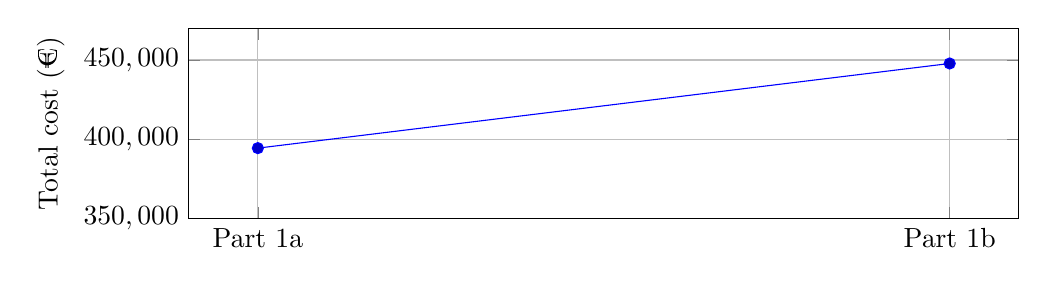
\begin{tikzpicture}
\begin{axis}[
    height=4cm,
    width=\textwidth,
    ymin=350000,
    ymax=470000,
    xtick={1,2},
    xticklabels={Part 1a, Part 1b},
    ylabel={Total cost (€)},
    grid=both,
    scaled y ticks=false,
    yticklabel style={
        /pgf/number format/fixed,
        /pgf/number format/1000 sep={,}
    }
]
\addplot+[mark=*] coordinates {
    (1,394454)
    (2,447792)
};
\end{axis}
\end{tikzpicture}
\end{minipage}
\caption{Cost comparison between part 1a and part 1b}
\end{table}

\assignmentsection{Assignment 2: Adjusting the MIP model with finite production capacity}

The objective of assignment 2 is to extend the model from assignment 1 by incorporating finite production capacity. In contrast to assignment 1, where production capacity was assumed to be unlimited, the production system is now constrained by the availability of two workstations.

\subsection{Plan based on forecasted demand}

\subsubsection{New capacity constraints}

Starting from the model in assignment 1a, two additional capacity constraints are introduced, one for each workstation. The inventory balance constraint, setup linking constraint and minimum lot size constraint from assignment 1a remain unchanged. The additional restrictions only limit the maximum feasible production quantities in each period.

Workstation X is used for the production of the end product \(E2801\). Its maximum capacity equals 800 units per week. Therefore, the number of units of \(E2801\) started in production in a given week cannot exceed this weekly capacity:

\begin{align}
x_{E2801,t} &\leq 800
&& \forall t \in \{1,\ldots,30\}
\tag{4}
\end{align}

Workstation Y is used for parts \(B1401\) and \(B2302\). Producing one unit of \(B1401\) requires 3 minutes of processing time, while producing one unit of \(B2302\) requires 2 minutes. The workstation operates continuously during the week, except for an 80-minute maintenance break. Hence, the available capacity is:

\[
7 \cdot 24 \cdot 60 - 80 = 10{,}000 \text{ minutes per week}
\]

The corresponding capacity constraint for workstation Y is:

\begin{align}
3x_{B1401,t} + 2x_{B2302,t} &\leq 10{,}000
&& \forall t \in \{1,\ldots,30\}
\tag{5}
\end{align}

The complete model for assignment 2a is therefore the model from assignment 1a, extended with constraints (4) and (5). These capacity constraints restrict the timing of production and prevent the optimizer from producing arbitrarily large batches in a single period.

\subsubsection{Cost comparison}
Compared with assignment 1a, the introduction of finite production capacity leads to a significant increase in total cost, rising from €394{,}454.00 to €540{,}488.80. This increase is primarily driven by a substantial rise in setup costs, which grow from €79{,}500.00 to €145{,}500.00 (+83\%). Under capacity limitations, the model can no longer concentrate production in a few large batches during the most cost-efficient periods. Instead, production must be spread over more periods, resulting in smaller and more frequent production runs and therefore more setups.

In addition, holding costs increase from €314{,}954.00 to €394{,}988.80 (+25.4\%). This is because capacity constraints force production to occur earlier than in the infinite-capacity case, leading to higher inventory levels that must be carried over time.

Overall, the inclusion of capacity constraints reduces production flexibility, which increases both setup and holding costs. Although this results in a higher total cost, it produces a more realistic and operationally feasible production plan.

\begin{table}[H]
\centering
\begin{minipage}[c]{0.44\textwidth}
\centering
\begin{tabular}{lrr}
\toprule
\textbf{Cost comparison} & \textbf{Part 1a (€)} & \textbf{Part 2a (€)} \\
\midrule
Holding cost   & €314{,}954.00 & €394{,}988.80 \\
Setup cost     & €79{,}500.00  & €145{,}500.00 \\
Backorder cost & --            & -- \\
\midrule
\textbf{Total cost} & \textbf{€394{,}454.00} & \textbf{€540{,}488.80} \\
\bottomrule
\end{tabular}
\end{minipage}
\hspace{0.06\textwidth}
\begin{minipage}[c]{0.44\textwidth}
\centering
\textbf{Cost comparison}

\vspace{0.3em}
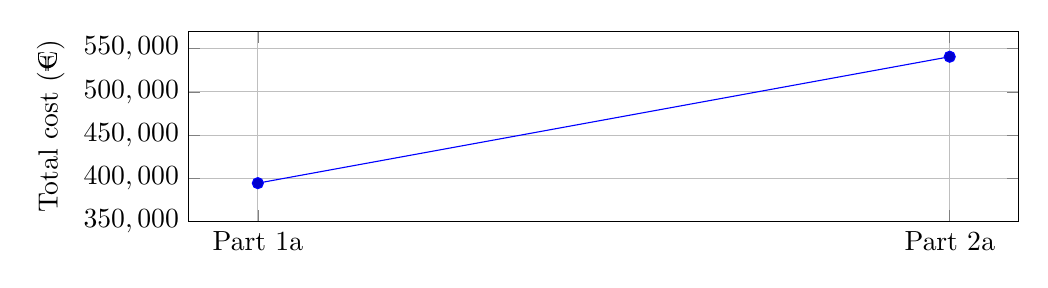
\begin{tikzpicture}
\begin{axis}[
    height=4cm,
    width=\textwidth,
    ymin=350000,
    ymax=570000,
    xtick={1,2},
    xticklabels={Part 1a, Part 2a},
    ylabel={Total cost (€)},
    grid=both,
    scaled y ticks=false,
    yticklabel style={
        /pgf/number format/fixed,
        /pgf/number format/1000 sep={,}
    }
]
\addplot+[mark=*] coordinates {
    (1,394454)
    (2,540488.80)
};
\end{axis}
\end{tikzpicture}
\end{minipage}
\caption{Cost comparison between assignment 1a and assignment 2a}
\end{table}

\subsection{Plan used on realized demand}

In part 2b, the production plan obtained in part 2a is evaluated using the realized demand instead of the forecasted demand. The production schedule remains unchanged, meaning that no re-optimization is performed. As a result, the setup cost stays identical at €145{,}500.00. The holding cost increases slightly from €394{,}988.80 to €401{,}114.80 due to deviations between forecasted and actual demand. In addition, backorder costs of €27{,}500.00 arise, indicating that the plan is not able to fully absorb demand variability under capacity constraints.

The service performance of the plan can be measured through the service level and the fill rate. The service level is 96.67\%, meaning that in 29 out of the 30 weeks there is no backorder at the end of the period. The fill rate equals 98.17\%, which indicates that almost all demanded units are delivered on time. Hence, the plan performs very well in terms of service, despite being constructed under capacity limitations.

Backorders only occur in week 30, where a shortage of 110 units arises. This shows that the plan is generally robust, but still vulnerable in periods where demand peaks exceed the available capacity and inventory buffers.

Overall, the total cost increases from €540{,}488.80 to €574{,}114.80. Compared to assignment 1b, the backorder cost is lower, suggesting that the finite capacity plan is slightly more robust against demand fluctuations.

However, shortages still occur, showing that capacity constraints limit the flexibility to respond to higher-than-expected demand.

\begin{table}[H]
\centering
\begin{minipage}[c]{0.44\textwidth}
\centering
\begin{tabular}{lrr}
\toprule
\textbf{Cost comparison} & \textbf{Part 2a} & \textbf{Part 2b} \\
\midrule
Holding cost   & €394{,}988.80 & €401{,}114.80 \\
Set-up cost    & €145{,}500.00 & €145{,}500.00 \\
Backorder cost & --            & €27{,}500.00 \\
\midrule
\textbf{Total cost} & \textbf{€540{,}488.80} & \textbf{€574{,}114.80} \\
\bottomrule
\end{tabular}
\end{minipage}
\hspace{0.06\textwidth}
\begin{minipage}[c]{0.44\textwidth}
\centering
\textbf{Cost comparison}

\vspace{0.3em}
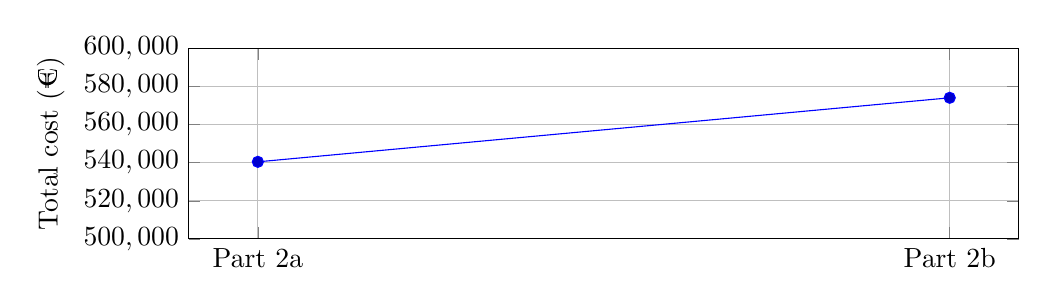
\begin{tikzpicture}
\begin{axis}[
    height=4cm,
    width=\textwidth,
    ymin=500000,
    ymax=600000,
    xtick={1,2},
    xticklabels={Part 2a, Part 2b},
    ylabel={Total cost (€)},
    grid=both,
    scaled y ticks=false,
    yticklabel style={
        /pgf/number format/fixed,
        /pgf/number format/1000 sep={,}
    }
]
\addplot+[mark=*] coordinates {
    (1,540488.80)
    (2,574114.80)
};
\end{axis}
\end{tikzpicture}
\end{minipage}
\caption{Comparison part 2a and 2b}
\end{table}

\assignmentsection{Assignment 3: Adjusting the MIP model to overtime}

\subsection{Plan based on forecasted demand}

In this assignment, the model from Assignment 2a is extended by introducing the possibility of overtime, also called temporary capacity expansion. Unlike the fixed capacity constraints in Assignment 2, this extension allows the company to increase capacity in specific periods at an additional cost, thereby improving flexibility.

\subsubsection{Decision variables}

We add two decision variables to the objective function that will represent the overtime for each workstation.

\begin{itemize}
    \item \(OT_{X,t}\): additional capacity in units for workstation X in period \(t\)
    \item \(OT_{Y,t}\): additional capacity in hours for workstation Y in period \(t\)
\end{itemize}

\subsubsection{Parameters}

\begin{itemize}
    \item \(c_{OTX}\): €2 per additional unit of capacity for workstation X
    \item \(c_{OTY}\): €120 per additional hour of capacity for workstation Y
\end{itemize}

\subsubsection{Objective function}

\[
\min \sum_{t=1}^{T=30} \sum_{i \in parts}
\left(
h_i I_{i,t}
+ S_i y_{i,t}
+ c_{OTX} OT_{X,t}
+ c_{OTY} OT_{Y,t}
\right)
\]

\subsubsection{Constraints}

The first three constraints remain identical to the base model from Assignment 1a:

\begin{itemize}[noitemsep, topsep=0pt]
    \item Constraint 1: inventory balance constraint
    \item Constraint 2: setup linking constraint
    \item Constraint 3: minimum lot size constraint
\end{itemize}

The overtime model adds two additional types of constraints.

\textbf{Constraint 4: capacity constraints with overtime}

For workstation X, the production of the end product \(E2801\) in each period cannot exceed the regular weekly capacity of 800 units plus the additional overtime capacity \(OT_{X,t}\).

\[
x_{E2801,t} \leq 800 + OT_{X,t}
\qquad
\forall t \in \{1,\ldots,30\}
\]

For workstation Y, the total processing time of parts \(B1401\) and \(B2302\) cannot exceed the regular weekly capacity of 10{,}000 minutes plus the overtime capacity. Since \(OT_{Y,t}\) is expressed in hours, it is multiplied by 60 to convert it into minutes.

\[
3x_{B1401,t} + 2x_{B2302,t}
\leq 10{,}000 + 60OT_{Y,t}
\qquad
\forall t \in \{1,\ldots,30\}
\]

\textbf{Constraint 5: maximum overtime limits}

The overtime variables are also bounded. Workstation X can use at most 300 additional units of capacity per week, while workstation Y can use at most 38 additional hours per week.

\[
OT_{X,t} \leq 300
\qquad
\forall t \in \{1,\ldots,30\}
\]

\[
OT_{Y,t} \leq 38
\qquad
\forall t \in \{1,\ldots,30\}
\]

\subsubsection{Cost comparison}

The introduction of overtime reduces the total cost by approximately €19{,}000 (-3.6\%) compared to production without overtime. This reduction is driven by the increased flexibility in capacity, which allows the system to better respond to fluctuations in demand. Additionally, the need for inventory buffers is reduced, as production can be more closely aligned with demand peaks instead of relying on early production and stock buildup.
Additionally, note that the Gurobi optimizer also identified an alternative optimal solution with the same total cost. This solution differs slightly in the distribution between holding costs and overtime costs, reflecting a different production schedule. However, since the total cost remains identical, we retain this solution.

\begin{table}[H]
\centering
\begin{minipage}[c]{0.44\textwidth}
\centering
\begin{tabular}{lrr}
\toprule
\textbf{Cost Comparison} & \textbf{Part 2a} & \textbf{Part 3a} \\
\midrule
Holding Cost   & €394{,}988.80 & €369{,}328.80 \\
Set-up Cost    & €145{,}500.00 & €145{,}500.00 \\
Backorder Cost & --            & -- \\
Overtime Cost  & --            & €6{,}442.00 \\
\midrule
\textbf{Total Cost} & \textbf{€540{,}488.80} & \textbf{€521{,}270.80} \\
\bottomrule
\end{tabular}
\end{minipage}
\hspace{0.06\textwidth}
\begin{minipage}[c]{0.44\textwidth}
\centering
\textbf{Cost comparison}

\vspace{0.3em}
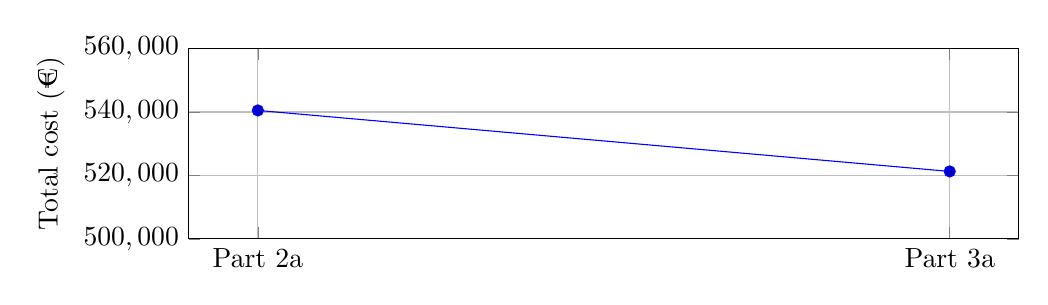
\begin{tikzpicture}
\begin{axis}[
    height=4cm,
    width=\textwidth,
    ymin=500000,
    ymax=560000,
    xtick={1,2},
    xticklabels={Part 2a, Part 3a},
    ylabel={Total cost (€)},
    grid=both,
    scaled y ticks=false,
    yticklabel style={
        /pgf/number format/fixed,
        /pgf/number format/1000 sep={,}
    }
]
\addplot+[mark=*] coordinates {
    (1,540488.80)
    (2,521270.80)
};
\end{axis}
\end{tikzpicture}
\end{minipage}
\caption{Comparison part 2a and 3a}
\end{table}

\subsection{Plan used on realized demand}

In part 3b, the production plan obtained in part 3a is evaluated using the realized demand instead of the forecasted demand. The production schedule and the overtime decisions remain unchanged, meaning that no re-optimization is performed. As a result, the setup cost stays identical at €145{,}500.00 and the total overtime cost remains €6{,}442.00. The holding cost increases from €369{,}328.80 to €375{,}610.80 due to deviations between forecasted and realized demand. In addition, backorder costs of €34{,}000.00 arise, indicating that the plan is not able to fully absorb demand variability, even with the overtime capacity included in the original plan.

The service performance of the plan can be measured through the service level and the fill rate. The service level is 93.33\%, meaning that in 28 out of the 30 weeks there is no backorder at the end of the period. The fill rate equals 97.74\%, which indicates that 5{,}881 out of 6{,}017 demanded units are delivered on time. Hence, the plan still performs well in terms of service, but realized demand causes shortages in some periods.

Backorders occur in week 26 and week 30, with shortages of 26 and 110 units respectively. This shows that the overtime plan improves production flexibility compared to the strict finite-capacity case, but it does not completely eliminate the effect of demand uncertainty.

Overall, the total cost increases from €521{,}270.80 to €561{,}552.80, corresponding to an increase of €40{,}282.00. This increase is mainly caused by the introduction of backorder costs and a higher holding cost, while setup and overtime costs remain unchanged.

\begin{table}[H]
\centering
\begin{minipage}[c]{0.44\textwidth}
\centering
\begin{tabular}{lrr}
\toprule
\textbf{Cost comparison} & \textbf{Part 3a} & \textbf{Part 3b} \\
\midrule
Holding cost   & €369{,}328.80 & €375{,}610.80 \\
Set-up cost    & €145{,}500.00 & €145{,}500.00 \\
Overtime cost  & €6{,}442.00   & €6{,}442.00 \\
Backorder cost & --            & €34{,}000.00 \\
\midrule
\textbf{Total cost} & \textbf{€521{,}270.80} & \textbf{€561{,}552.80} \\
\bottomrule
\end{tabular}
\end{minipage}
\hspace{0.06\textwidth}
\begin{minipage}[c]{0.44\textwidth}
\centering
\textbf{Cost comparison}

\vspace{0.3em}
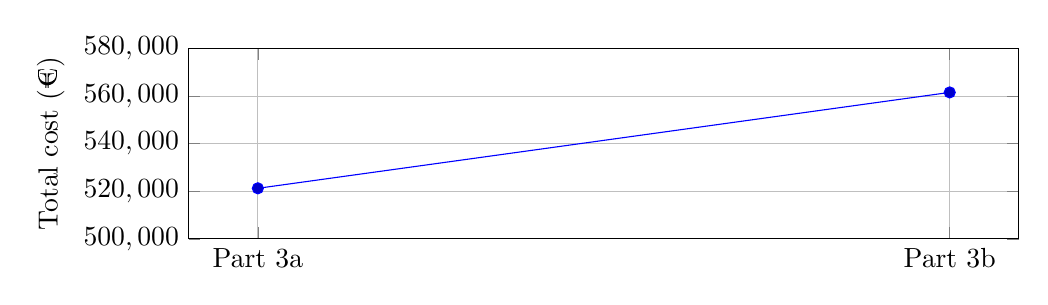
\begin{tikzpicture}
\begin{axis}[
    height=4cm,
    width=\textwidth,
    ymin=500000,
    ymax=580000,
    xtick={1,2},
    xticklabels={Part 3a, Part 3b},
    ylabel={Total cost (€)},
    grid=both,
    scaled y ticks=false,
    yticklabel style={
        /pgf/number format/fixed,
        /pgf/number format/1000 sep={,}
    }
]
\addplot+[mark=*] coordinates {
    (1,521270.80)
    (2,561552.80)
};
\end{axis}
\end{tikzpicture}
\end{minipage}
\caption{Cost comparison part 3a and 3b}
\end{table}

\subsubsection{Additional sensitivity insight}

The previous evaluation assumes that the production plan and the overtime decisions from part 3a remain fixed when realized demand occurs. Under this assumption, backorders still arise in weeks 26 and 30, leading to a backorder cost of €34{,}000.00. However, an additional sensitivity analysis was performed to examine what would happen if overtime capacity could be adjusted after observing realized demand.

This scenario requires an important operational assumption. It assumes that the realized demand is known sufficiently early, for example at the beginning of the week, and that the company is flexible enough to still adapt overtime decisions before production is executed. This is not the same as assuming instantaneous reaction with zero time delay, which would be unrealistic. Rather, it represents a short-term flexible planning environment in which overtime can still be scheduled in response to updated demand information.

Under this assumption, the remaining overtime capacity is sufficient to absorb the demand deviations. The model can eliminate all backorders by using additional overtime, resulting in a service level and fill rate of 100\%. In this sensitivity scenario, the total cost equals €538{,}767.00. This is higher than the forecast-based 3a cost of €521{,}270.80, but lower than the fixed-plan realized-demand evaluation in 3b, which resulted in a total cost of €561{,}552.80. The improvement is mainly caused by eliminating the €34{,}000.00 backorder cost, while only €442.00 of overtime cost is required.

This indicates that overtime capacity has value not only as a planned capacity expansion, but also as a short-term flexibility buffer against demand uncertainty. Nevertheless, this interpretation depends strongly on the assumption that overtime decisions can still be adjusted after demand becomes known. If overtime must be fixed in advance together with the production plan, then the original 3b evaluation remains the more realistic comparison.

For a more detailed insight into the results, we refer to the Excel file \texttt{OUTPUT.xlsx}.

\assignmentsection{Assignment 4: Adjusting the MIP model with machine expansion}

In this chapter, the production planning model is extended to allow the company to permanently increase the capacity of its two workstations through machine modernisation. Unlike the overtime option explored in Assignment 3, this expansion represents a one-time capital investment that raises the capacity ceiling for every period in the planning horizon. The goal is to determine the cost-optimal level of expansion and evaluate whether the investment pays off under both forecasted and realised demand.

\subsection{Plan based on forecasted demand}

For Assignment 4a, we build upon the finite capacity MIP model developed in Assignment 2a, which already incorporates the production planning constraints for both workstations alongside the inventory balance, minimum lot size, and Big-M constraints. To extend this model with the possibility of permanent capacity expansion, two new decision variables and four new parameters are introduced.

\subsubsection{Decision variables}

\begin{itemize}
    \item \(dx\): represents the number of additional units permanently added to the capacity of Workstation X, and is bounded between 0 and 200.
    \item \(dy\_pct\): represents the number of 1\%-increment steps by which the capacity of Workstation Y is permanently increased, bounded between 0 and 40, corresponding to a maximum expansion of 40\%.
\end{itemize}

\subsubsection{Parameters}

\begin{itemize}
    \item \(COST^{EXP}_{X}\): €10 cost per additional unit of capacity added to Workstation X.
    \item \(COST^{EXP}_{Y}\): €1500 cost per 1\% increment of additional capacity on Workstation Y.
\end{itemize}

\subsubsection{Objective function}

The two new decision variables are independent of the period, since we determine once at the beginning how much the capacity increase will be. In our objective function, we multiply this amount of minutes with the cost per minute.

\[
\min \sum_{t=1}^{T=30} \sum_{i \in parts}
\left(h_i I_{i,t} + S_i y_{i,t}\right)
+ COST^{EXP}_{X} \cdot dx
+ COST^{EXP}_{Y} \cdot dy\_pct
\]

\subsubsection{Constraints}

The model extends the base formulation from Assignment 1a. Therefore, the following constraints remain unchanged:

\begin{itemize}[noitemsep]
    \item Constraint 1: inventory balance constraint (1a)
    \item Constraint 2: setup constraint (1a)
    \item Constraint 3: minimum lot size constraint (1a)
\end{itemize}

\textbf{Constraint 4: Capacity constraints with expansion}

Two capacity constraints are introduced, one for each workstation. These constraints ensure that production in each period does not exceed the available capacity, which can now be permanently increased through expansion decisions.

\begin{itemize}
    \item \textit{Workstation X (end product $E2801$):} \\
    The production of the end product in each period is limited by the base capacity of 800 units, which can be increased by the expansion variable $dx$.
\end{itemize}

\[
x_{E2801,t} \leq 800 + dx 
\qquad \forall t \in \{1,\ldots,30\}
\]

\begin{itemize}
    \item \textit{Workstation Y (components $B1401$ and $B2302$):} \\
    The total processing time required for component production is constrained by the available capacity in minutes. This capacity can be increased proportionally through the expansion variable $dy\_pct$.
\end{itemize}

\[
3x_{B1401,t} + 2x_{B2302,t}
\leq 10{,}000 + 100 \cdot dy\_pct
\qquad \forall t \in \{1,\ldots,30\}
\]

\textbf{Constraint 5: Expansion limits}

These constraints ensure that the expansion decisions remain within feasible and predefined bounds.

\begin{itemize}
    \item The capacity expansion of workstation X is limited to at most 200 additional units.
    \item The capacity expansion of workstation Y is limited to at most 40\%, expressed in discrete percentage steps.
\end{itemize}

\[
0 \leq dx \leq 200
\]

\[
0 \leq dy\_pct \leq 40
\]

\subsubsection{Cost comparison}

Part 2a results in the highest total cost (€540{,}488.80) due to high holding and setup costs under strict capacity constraints. In Part 3a, allowing overtime reduces the total cost to €521{,}270.80 by lowering holding costs, although it introduces additional overtime costs. Part 4a achieves the lowest total cost (€520{,}723.30) by enabling permanent capacity expansion. Despite the added investment cost, this option further reduces holding and setup costs, making it the most cost-efficient solution overall.

\begin{table}[H]
\centering
\begin{minipage}[c]{0.50\textwidth}
\centering
\resizebox{\linewidth}{!}{
\begin{tabular}{lrrr}
\toprule
\textbf{Cost comparison} & \textbf{Part 2a} & \textbf{Part 3a} & \textbf{Part 4a} \\
\midrule
Holding Cost   & €394{,}988.80 & €369{,}328.80 & €364{,}253.30 \\
Set-Up cost    & €145{,}500.00 & €145{,}500.00 & €143{,}000.00 \\
Overtime Cost  & --            & €6{,}442.00   & -- \\
Expansion Cost & --            & --            & €13{,}470.00 \\
Backorder Cost & --            & --            & -- \\
\midrule
\textbf{Total Cost} & \textbf{€540{,}488.80} & \textbf{€521{,}270.80} & \textbf{€520{,}723.30} \\
\bottomrule
\end{tabular}
}
\end{minipage}
\hspace{0.03\textwidth}
\begin{minipage}[c]{0.42\textwidth}
\centering
\textbf{Cost comparison}

\vspace{0.3em}
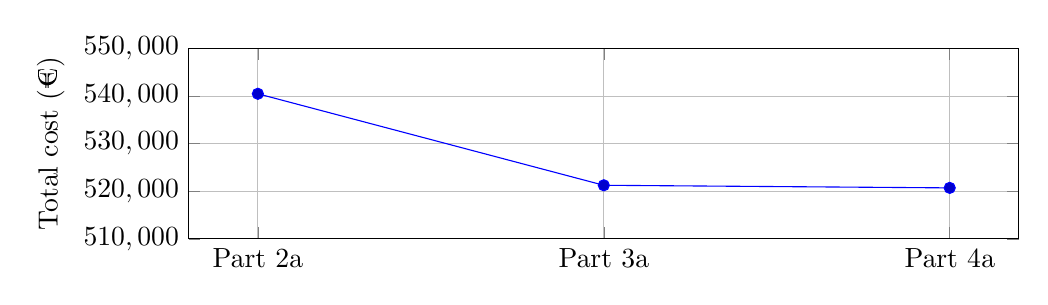
\begin{tikzpicture}
\begin{axis}[
    height=4cm,
    width=\textwidth,
    ymin=510000,
    ymax=550000,
    xtick={1,2,3},
    xticklabels={Part 2a, Part 3a, Part 4a},
    ylabel={Total cost (€)},
    grid=both,
    scaled y ticks=false,
    yticklabel style={
        /pgf/number format/fixed,
        /pgf/number format/1000 sep={,}
    }
]
\addplot+[mark=*] coordinates {
    (1,540488.80)
    (2,521270.80)
    (3,520723.30)
};
\end{axis}
\end{tikzpicture}
\end{minipage}
\caption{Cost comparison part 2a, 3a and 4a}
\end{table}

\subsection{Plan based on realized demand}

In part 4b, the production plan obtained in part 4a is evaluated using the realized demand instead of the forecasted demand. Again no re-optimization is performed. As a result, the setup cost stays identical at €143{,}000.00 and the expansion cost remains €13{,}470.00. The holding cost increases slightly from €364{,}253.30 to €370{,}457.30 due to deviations between forecasted and actual demand. In addition, backorder costs of €30{,}750.00 arise, indicating that the plan is not able to fully absorb demand variability despite the increased capacity.

The service level is 93.33\%, meaning that in 28 out of the 30 weeks there is no backorder at the end of the period. The fill rate equals 97.96\%, indicating that the majority of demand is satisfied on time, although slightly less compared to previous scenarios.

Backorders only occur in week 26 and week 30, where shortages of 13 and 110 units arise respectively. This shows that even with expanded capacity, the system remains vulnerable to demand peaks that exceed both capacity and available inventory buffers.

Overall, the total cost increases from €520{,}723.30 to €557{,}677.30. This increase is mainly driven by the introduction of backorder costs, while setup and expansion costs remain unchanged. Compared to assignment 2b, the total cost is lower, indicating that capacity expansion helps reduce overall costs. However, shortages still occur, indicating that expansion alone is not sufficient to fully hedge against demand uncertainty.

\begin{table}[H]
\centering
\begin{minipage}[c]{0.44\textwidth}
\centering
\begin{tabular}{lrr}
\toprule
\textbf{Cost comparison} & \textbf{Part 4a} & \textbf{Part 4b} \\
\midrule
Holding Cost   & €364{,}253.30 & €370{,}457.30 \\
Set-Up cost    & €143{,}000.00 & €143{,}000.00 \\
Overtime Cost  & --            & -- \\
Expansion Cost & €13{,}470.00  & €13{,}470.00 \\
Backorder Cost & --            & €30{,}750.00 \\
\midrule
\textbf{Total Cost} & \textbf{€520{,}723.30} & \textbf{€557{,}677.30} \\
\bottomrule
\end{tabular}
\end{minipage}
\hspace{0.06\textwidth}
\begin{minipage}[c]{0.44\textwidth}
\centering
\textbf{Cost comparison}

\vspace{0.3em}
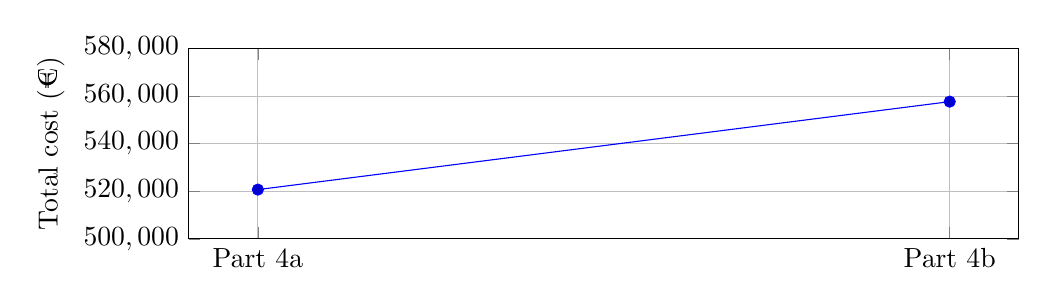
\begin{tikzpicture}
\begin{axis}[
    height=4cm,
    width=\textwidth,
    ymin=500000,
    ymax=580000,
    xtick={1,2},
    xticklabels={Part 4a, Part 4b},
    ylabel={Total cost (€)},
    grid=both,
    scaled y ticks=false,
    yticklabel style={
        /pgf/number format/fixed,
        /pgf/number format/1000 sep={,}
    }
]
\addplot+[mark=*] coordinates {
    (1,520723.30)
    (2,557677.30)
};
\end{axis}
\end{tikzpicture}
\end{minipage}
\caption{Cost comparison part 4a and 4b}
\end{table}

\assignmentsection{Assignment 5: Adjusting the MIP model with overtime and machine expansion}

In this assignment, the MIP model is extended by combining both overtime and permanent capacity expansion. This allows the model to choose between short-term flexibility, overtime, and long-term structural improvements, capacity expansion, or a combination of both.

\subsection{Plan based on forecasted demand}

The model of Part 5 is based on the model of Part 2a. Because Part 5 combines the adjustments of part 3a and 4a, a lot of things return from those models when adding the extra info to the base model.

\subsubsection{Parameters}

We combine the added parameters from assignment 3 and 4 and we add these to the base model from assignment 2.

\begin{itemize}
    \item \(c_{OTX}\): €2 per additional unit of capacity for workstation X
    \item \(c_{OTY}\): €120 per additional hour of capacity for workstation Y
    \item \(COST^{EXP}_{X}\): €10 cost per additional unit of capacity added to Workstation X
    \item \(COST^{EXP}_{Y}\): €1500 cost per 1\% increment of additional capacity on Workstation Y
\end{itemize}

\subsubsection{Objective function}

\[
\min \sum_{t=1}^{T=30} \sum_{i \in parts}
\left(
h_i I_{i,t}
+ S_i y_{i,t}
+ c_{OTX} OT_{X,t}
+ c_{OTY} OT_{Y,t}
\right)
+ COST^{EXP}_{X} \cdot dx
+ COST^{EXP}_{Y} \cdot dy\_pct
\]

\subsubsection{Constraints}

Constraint 1: inventory balance constraint (1a) \\
Constraint 2: setup constraint (1a) \\
Constraint 3: minimum lot size constraint (1a) \\
Constraint 4: maximum overtime (3a) \\
Constraint 5: maximum expansion (4a)

Constraint 6: maximum capacity adjusted with overtime and permanent expansion for both workstations

This first new constraint ensures that the production of the end product \(E2801\) in each period does not exceed the total available capacity of workstation X, which consists of the base capacity, the temporary increase through overtime \(OT_{X,t}\), and the permanent capacity expansion \(dx\).

\[
x_{E2801,t} \leq 800 + OT_{X,t} + dx
\qquad
\forall t \in \{1,\ldots,30\}
\]


The second constraint limits the total processing time required on workstation Y by considering the processing times of components \(B1401\) and \(B2302\), while allowing capacity to be increased both temporarily through overtime \(OT_{Y,t}\) and structurally through a percentage-based expansion \(dy\_pct\).

\[
3x_{B1401,t} + 2x_{B2302,t}
\leq 10{,}000 + 60OT_{Y,t} + 100 \cdot dy\_pct
\qquad
\forall t \in \{1,\ldots,30\}
\]

\subsubsection{Cost comparison}

We observe that a combination of working overtime and machine expansion decreases the total cost. Next to that, all cost types separately are lower than previous parts. This could possibly be the best production plan so far. However, ``total cost'' is not our only performance measure. In part 5b, where we also take the real demand into consideration, we will also take a look at the fill rate to compare this production plan to the previous ones.

\begin{table}[H]
\centering
\begin{minipage}[c]{0.52\textwidth}
\centering
\resizebox{\linewidth}{!}{
\begin{tabular}{lrrrr}
\toprule
\textbf{Cost comparison} & \textbf{Part 2a} & \textbf{Part 3a} & \textbf{Part 4a} & \textbf{Part 5a} \\
\midrule
Holding Cost   & €394{,}988.80 & €369{,}328.80 & €364{,}253.30 & €354{,}296.60 \\
Set-Up Cost    & €145{,}500.00 & €145{,}500.00 & €143{,}000.00 & €132{,}000.00 \\
Overtime Cost  & --            & €6{,}442.00   & --            & €600.00 \\
Expansion Cost & --            & --            & €13{,}470.00  & €23{,}180.00 \\
Backorder Cost & --            & --            & --            & -- \\
\midrule
\textbf{Total Cost} & \textbf{€540{,}488.80} & \textbf{€521{,}270.80} & \textbf{€520{,}723.30} & \textbf{€510{,}076.60} \\
\bottomrule
\end{tabular}
}
\end{minipage}
\hspace{0.03\textwidth}
\begin{minipage}[c]{0.40\textwidth}
\centering
\textbf{Cost comparison}

\vspace{0.3em}
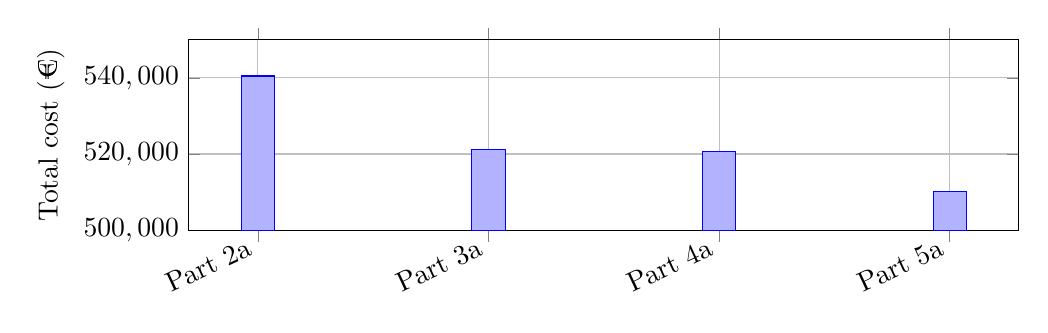
\begin{tikzpicture}
\begin{axis}[
    height=4cm,
    width=\textwidth,
    ymin=500000,
    ymax=550000,
    ybar,
    bar width=12pt,
    xtick=data,
    xticklabels={Part 2a, Part 3a, Part 4a, Part 5a},
    ylabel={Total cost (€)},
    grid=both,
    scaled y ticks=false,
    yticklabel style={
        /pgf/number format/fixed,
        /pgf/number format/1000 sep={,}
    },
    x tick label style={rotate=25, anchor=east}
]
\addplot coordinates {
    (1,540488.80)
    (2,521270.80)
    (3,520723.30)
    (4,510076.60)
};
\end{axis}
\end{tikzpicture}
\end{minipage}
\caption{Comparison part 2a, 3a, 4a and 5a}
\end{table}

\subsection{Plan based on realized demand}

In part 5b, the production plan obtained in part 5a is evaluated using the realized demand instead of the forecasted demand. The production schedule, as well as the chosen capacity expansions and overtime decisions, remain unchanged, meaning that no re-optimization is performed. As a result, the setup cost stays identical at €132{,}000.00, the expansion cost remains €23{,}180.00, and the overtime cost stays €600.00. The holding cost increases slightly from €354{,}296.60 to €360{,}656.60 due to deviations between forecasted and actual demand. In addition, backorder costs of €37{,}250.00 arise, indicating that even with both overtime and permanent capacity expansion, the plan cannot fully absorb demand variability.

The service performance of the plan can be measured through the service level and the fill rate. The service level is 93.33\%, meaning that in 28 out of the 30 weeks there is no backorder at the end of the period. The fill rate equals 97.52\%, which indicates that 5{,}868 out of 6{,}017 demanded units are delivered on time. Hence, the plan performs well, but slightly worse compared to some previous scenarios in terms of service robustness.

Backorders only occur in week 26 and week 30, where shortages of 39 and 110 units arise respectively. This shows that even with the combination of overtime and capacity expansion, the system remains sensitive to peak demand periods where available capacity and inventory buffers are insufficient.

Overall, the total cost increases from €510{,}076.60 to €553{,}686.60. This increase is mainly driven by the introduction of backorder costs, while setup, expansion, and overtime costs remain unchanged.

Compared with assignment 4b, the total cost is slightly lower, indicating that combining overtime with expansion improves cost efficiency. However, the presence of backorders shows that even this more flexible strategy does not fully eliminate the impact of demand uncertainty.

\begin{table}[H]
\centering
\begin{minipage}[c]{0.44\textwidth}
\centering
\begin{tabular}{lrr}
\toprule
\textbf{Cost comparison} & \textbf{Part 5a} & \textbf{Part 5b} \\
\midrule
Holding Cost   & €354{,}296.60 & €360{,}656.60 \\
Set-Up Cost    & €132{,}000.00 & €132{,}000.00 \\
Overtime Cost  & €600.00       & €600.00 \\
Expansion Cost & €23{,}180.00  & €23{,}180.00 \\
Backorder Cost & --            & €37{,}250.00 \\
\midrule
\textbf{Total Cost} & \textbf{€510{,}076.60} & \textbf{€553{,}686.60} \\
\bottomrule
\end{tabular}
\end{minipage}
\hspace{0.06\textwidth}
\begin{minipage}[c]{0.44\textwidth}
\centering
\textbf{Cost comparison}

\vspace{0.3em}
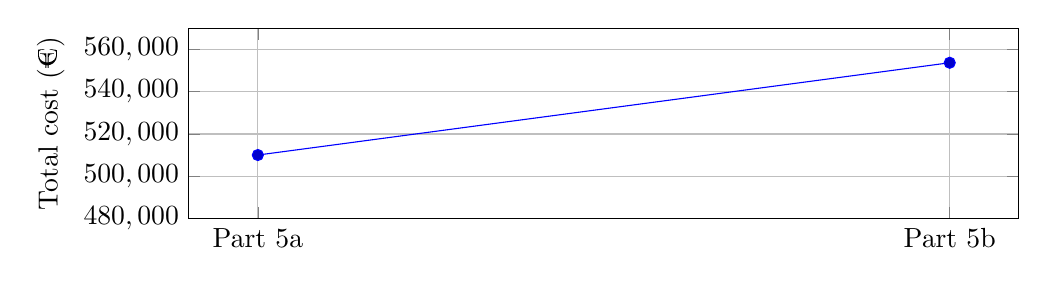
\begin{tikzpicture}
\begin{axis}[
    height=4cm,
    width=\textwidth,
    ymin=480000,
    ymax=570000,
    xtick={1,2},
    xticklabels={Part 5a, Part 5b},
    ylabel={Total cost (€)},
    grid=both,
    scaled y ticks=false,
    yticklabel style={
        /pgf/number format/fixed,
        /pgf/number format/1000 sep={,}
    }
]
\addplot+[mark=*] coordinates {
    (1,510076.60)
    (2,553686.60)
};
\end{axis}
\end{tikzpicture}
\end{minipage}
\caption{Cost comparison part 5a and 5b}
\end{table}

\assignmentsection{Assignment 6:  Adjusting the MIP model with creative ideas}


Starting from the model in Part 5, we sought ways to enhance its performance using real demand data, particularly in managing the disparity between forecasted and realized demand, or uncertainty.

\subsection{6a. Ideas to improve performance and reduce uncertainty}

\textbf{Idea 1: Working with a safety stock}

To account for demand uncertainty, a safety stock was introduced for the end product (Lim\`{e}re, 2026). In the previous assignments, the production plan was optimized based on forecasted demand only. However, as observed in the dataset, the realized demand consistently deviates from the forecast, which may lead to stockouts and consequently backorder costs. To mitigate this risk, a safety stock policy was implemented.

The safety stock level was determined using a standard statistical approach based on forecast errors. The forecast error per period was calculated as the difference between realized and forecasted demand. The standard deviation of these errors ($\sigma_e$) was then computed to quantify the variability in demand:

\begin{equation}
    \sigma_e = \text{std}(d_t^{\text{realized}} - d_t^{\text{forecast}}), \quad t \in \{1, \dots, 30\}
\end{equation}

A first, simplified approach computes the safety stock directly from the forecast error standard deviation:

\begin{equation}
    SS = z_{1-\alpha} \cdot \sigma_e
\end{equation}

This formulation assumes that the safety stock only needs to cover the variability within a single period. However, the system operates with a lead time of $L = 1$ period for the end product and a weekly review period of $R = 1$. The lead time refers to the delay between placing a production order and receiving the finished goods; the review period reflects how frequently production decisions are made. During this combined window of $L + R = 2$ periods, no corrective action can be taken, meaning the safety stock must absorb all demand fluctuations that occur within this interval. Accounting for this, the standard deviation over the full uncertainty window becomes:

\begin{equation}
    \sigma_{LTD} = \sigma_e \cdot \sqrt{L + R}
\end{equation}

The resulting safety stock is then:

\begin{equation}
    SS = z_{1-\alpha} \cdot \sigma_{LTD}
\end{equation}

This safety stock was incorporated into the MIP model as a lower bound on the inventory of the end product in each period:

\begin{equation}
    I_{E2801,t} \geq SS \quad \forall t \in \{1, \dots, T\}
\end{equation}

By enforcing this constraint, the model is forced to maintain a buffer against demand variability, which shifts production earlier in time and reduces the likelihood of stockouts when realized demand exceeds the forecast. Compared to the model without safety stock, this approach typically leads to higher holding costs due to the additional inventory. However, under realized demand, safety stock effectively buffers against demand variability, significantly reducing backorders and their associated costs. Given the relatively high backorder cost in this problem setting, maintaining a safety stock is economically justified and results in a more robust production plan under uncertainty.

To assess the sensitivity of this approach to the chosen confidence level, the model was solved under two target cycle service levels: 95\% ($z_{1-\alpha} = 1.65$, $SS = 60$ units) and 99\% ($z_{1-\alpha} = 2.33$, $SS = 84$ units). The key results are summarized in Table~\ref{tab:ss_results}. A full cost breakdown and detailed production schedules can be found in the accompanying Excel file.

\begin{table}[h]
    \centering
    \caption{Safety stock sensitivity analysis: key results}
    \label{tab:ss_results}
    \begin{tabular}{l c c c c c}
        \toprule
        \textbf{Design} & \textbf{Safety Stock} & \textbf{Total Cost (forecast)} & \textbf{Total Cost (realized)} & \textbf{\# backorder} & \textbf{Service level} \\
        \midrule
        Assignment 5b & (No) & \texteuro 510,076.60 & \texteuro 553,686.60 & 149 & 93.33\% \\
        95\% CSL     & 60   & \texteuro 520,462.60 & \texteuro 538,728.60 & 50  & 96.67\% \\
        99\% CSL     & 84   & \texteuro 524,617.00 & \texteuro 536,739.00 & 26  & 96.67\% \\
        \bottomrule
    \end{tabular}
\end{table}

Both safety stock levels significantly reduce backorder costs under realized demand. Notably, the 99\% service level yields a lower total cost than the 95\% level under realized demand (\texteuro 536,739 vs.\ \texteuro 538,729). This counterintuitive result arises because the backorder penalty (\texteuro 250/unit/week) vastly exceeds the holding cost (\texteuro 6/unit/week for E2801). The additional 24 units of safety stock generate approximately \texteuro 1,850 in extra holding costs but prevent backorders worth approximately \texteuro 6,000, yielding a net saving of roughly \texteuro 4,150. This suggests that for this particular cost structure, even higher service levels could be economically beneficial.

\vspace{0.5em}
\textbf{Idea 2: Outsourcing production}

\vspace{0.5em}
\textbf{Idea 3: Double exponential smoothing for demand forecasting}

One candidate forecasting method to handle demand uncertainty is Holt's method (double exponential smoothing), which extends simple exponential smoothing by maintaining two smoothing equations: one for the level of the series ($S_t$) and one for the trend ($G_t$), controlled by two smoothing constants $\alpha$ and $\beta$ respectively. The $\tau$-step-ahead forecast is then given by $F_{t,t+\tau} = S_t + \tau G_t$, making it well-suited for data exhibiting a linear trend.

However, applying Holt's method to this problem is not appropriate for two reasons. First, the method requires historical demand data prior to the planning horizon to reliably initialize $S_0$ and $G_0$, typically through linear regression. This is data that is not available here, as the dataset only covers weeks 1 through 30 with no preceding observations. Second, inspecting the realized demand reveals no clear linear trend; demand fluctuates around a relatively stable mean, making the trend component unnecessary. For these reasons, simpler and more robust approaches are better suited to address the uncertainty between forecasted and realized demand in this setting.

\vspace{0.5em}
\textbf{Idea 4: Increasing the number of periods in the planning horizon}

\subsection{Conclusion 6a}

\subsection{6b. Other sources of uncertainty}

Although demand uncertainty was the primary focus of this project, a production system faces many additional sources of uncertainty. A useful theoretical lens is the Variability Law: increasing variability always degrades system performance, and since variability propagates through the production chain, reduction efforts should be placed as early as possible. The Buffering Law adds that any system facing variability must be buffered by some combination of inventory, capacity, and time. The models developed in Assignments 1 to 5 rely primarily on inventory as a buffer.

\vspace{0.5em}
\textbf{Process uncertainty}

A relevant internal source of uncertainty arises from product and process complexity. In this case, E2801 has a multi-level bill of materials involving seven distinct parts across three production levels, requiring multiple coordinated assembly steps. Each additional step introduces its own variability, and since these steps are sequentially dependent, delays or errors at one level propagate directly to the next. This risk is present across all assignments, but is most consequential in Assignments 1 and 2, where no capacity buffer exists to absorb disruptions. Reducing the number of components or simplifying the BOM structure would shorten lead times and decrease the probability of cascading errors, thereby lowering overall system variability.

Additionally, setup operations contribute to variability, as each setup introduces uncertainty in effective processing time. While fewer setups reduce setup costs, larger batch sizes may increase variability propagation, illustrating a trade-off between cost efficiency and operational robustness.

\vspace{0.5em}
\textbf{Capacity uncertainty}

Capacity uncertainty arises when available workstation capacity deviates from assumed levels due to machine outages or operational disruptions. In Assignment 2, both workstations operate at fixed capacity with no flexibility, making the system fully exposed to this risk. Assignments 3 and 5 partially mitigate this through overtime flexibility, which acts as a capacity buffer when disruptions occur. Assignments 4 and 5 go further by permanently expanding capacity, lowering baseline utilization and thereby reducing the nonlinear impact of outages.

Introducing rework processes or improving maintenance policies could further reduce the impact of capacity losses by shortening recovery times and stabilizing effective capacity levels.

\vspace{0.5em}
\textbf{Lead time uncertainty}

Lead time uncertainty arises when the actual time between ordering and receiving components deviates from assumed fixed values, due to supplier delays, transportation problems, or other disruptions. In this model, all lead times are treated as deterministic across all assignments. However, even modest variation in the lead time of critical components such as B4702 (5 periods) could prevent V6302 production from starting on time, propagating directly to E2801.

None of the models include a safety lead time buffer for purchased components, meaning this risk remains unmitigated across Assignments 1 to 5. Incorporating lead time buffers or working with more reliable suppliers would reduce both the average lead time and its variability, improving system robustness.

\vspace{0.5em}
\textbf{Supply-side uncertainty}

Beyond the modeled uncertainties, supply-side disruptions such as supplier reliability issues, quality defects, or yield losses can further impact system performance. Yield losses and rework reduce effective throughput below nominal capacity, tightening bottlenecks and potentially generating shortages that safety stock alone cannot absorb. This highlights the importance of combining different types of buffers (inventory, capacity, and time) rather than relying on a single mechanism.

\clearpage
\assignmentsection{References}

\begin{flushleft}
\setlength{\parindent}{0pt}
\setlength{\parskip}{0.4em}

\hangindent=1.5em
\hangafter=1
Limière, V. (2026). APM3\_ProductionPlanning\_GroupProject [Lecture slides, Advanced Production Management, Ghent University].

\hangindent=1.5em
\hangafter=1
Graves, S. C. (1999). Manufacturing planning and control (Working paper). Massachusetts Institute of Technology.

\hangindent=1.5em
\hangafter=1
Limière, V. (2026). APM4\_Inventory\_Deterministic [Lecture slides, Advanced Production Management, Ghent University].

\hangindent=1.5em
\hangafter=1
Limière, V. (2026). APM5\_Inventory\_Stochastic [Lecture slides, Advanced Production Management, Ghent University].

\end{flushleft}

\assignmentsection{Appendix}

\end{document}